
\section{Numerical Methods for Fractional Differential Equations}

Although we have focused on fractional differential equations which involved Riemann-Liouviille derivatives or Caputo derivatives up until this point, it turns out that in many cases the Gr{\"u}nwald-Letnikov definition is equivelent \cite{Podlubny1999}. This is a useful fact because the Gr{\"u}nwald-Letnikov definition can be used for numerical evaluation of fractional derivatives. 

To do this we first recal the definition
$$
    \rld{a}{t}{\alpha}{f}(t) = \lim_{h \lra 0} \frac{\fracdelta{a}{\alpha}{h}{f}(t)}{h^\alpha}
$$

where

$$
    \fracdelta{a}{\alpha}{h}{f}(t) = \sum_{j=0}^{\lfloor \frac{t-a}{h} \rfloor} (-1)^j {\alpha \choose j } f(t-jh).
$$

By essentially choosing some small value of $ h $ we can arrive at a reasonable numerical approximation of the Riemann-Liouville fractional derivative of a function $ f $ \cite{Podlubny1999}.

We can also use quadrature rules to numerically fractionally integrate and differentiate functions \cite{Podlubny1999}. We will, however, not investigate that approach further and instead fucus on this finite differences idea outlined above.

One of the things which sould become immediatly apparent from the above definitions is that at $ t $ goes far away from $ a $ the number of terms in the sum which defines $ \fracdelta{a}{\alpha}{h}{f}(t) $ grows with $ O(t-a) $. This is not the case for integer order derivatives and this particular fact introduces numerous problems which we will attempt to solve or mitigate in the following sections.

\subsection{A Parallel Adams-Moulton-Bashforth FDE Solver via Modern Task Based Concurrency}
In this section we aim to take the work of Diethelm in \cite{Diethelm2011} and apply modern task based concurrency approaches to improve performance and scalability. We do this first via an implementation in MONO (.NET) with C\# and then gain performance increases by using C++ and Intel\textsuperscript{{\textregistered}}'s Threading Building Blocks and then gain collosal performance increases by utilising NVIDIA\textsuperscript{{\textregistered}}'s CUDA\textsuperscript{{\textregistered}}. 

These performance increases can mitigate the issue that arose from the growth in the number of terms of the sum that defined $ \fracdelta{a}{\alpha}{h}{f}(t) $ but they do not fundamentally change the complexity class of the algorithms discussed.

\subsubsection{Explanation of the Adams-Moulton-Bashforth Method}

The method that we explain here is designed to solve fractional differential equations of the form,
\begin{align}
    \capder{0}{x}{\alpha}{y}(x) = f(x,y)
\end{align}
along with initial conditions 
\begin{align}
    y(0) = y_0, y'(0) = y_0^{(1)}, \ldots, y^{(\lceil \alpha \rceil)}(0) = y_0^{(\lceil \alpha \rceil)}.
\end{align}

We use an Adams-Moulton-Bashford method described in \cite{Diethelm2011}. Firstly we need to choose some time $ T $ for the interval  $ [0, T ] $ over which we will solve the differential equation and some number of steps to use $ N $. This allows us to define a step size $ h := T/N $ and therefore the gridpoints $ x_j = jh $. 

From that we can calculate the predictor approximation
\begin{align}
    \label{eq:AMB_Predictor}
    y_{j+1}^{P} = \sum_{k=0}^{\lceil \alpha \rceil - 1} \frac{x^k_{j+1}}{k!}y_0^{(k)} + h^\alpha \sum_{k=0}^j b_{j-k}f(x_k, y_k)
\end{align}
with coefficients $ b_\mu $ given by
\begin{align}
    \label{eq:AMB_y}
    b_\mu = \frac{(\mu + 1)^\alpha - \mu^\alpha}{\Gamma(\alpha + 1)}.
\end{align}

We then calculate the actual approximation of $ y_{j+1} $ with
\begin{align}
    y_{j+1} = \sum_{k=0}^{\lceil \alpha \rceil -1} \frac{x_{j+1}^{k}}{k!}y_0^{(k)} + h^\alpha \left( c_j f(x_0, y_0) + \sum_{k=1}^{j}a_{j-k}f(x_k,y_k) + \frac{f(x_{j+1}, y_{j+1}^P)}{\Gamma(\alpha + 2)}\right)
\end{align}
with coefficients $ a_\mu $ and $ c_\mu $ given by
\begin{align}
    a_\mu = \frac{(\mu + 2)^{\alpha + 1}-2(\mu + 1)^{\alpha + 1} + \mu^{\alpha + 1}}{\Gamma(\alpha + 2)}
\end{align}
and
\begin{align}
    c_\mu = \frac{u^{\alpha + 1} - (\mu - \alpha)(\mu + 1)^\alpha}{\Gamma(\alpha + 2)}.
\end{align}


As discussed in \cite{Diethelm2004} and \cite{Diethelm2011} this algorithm converges in the sense that
\begin{align}
    \max_{j=0,1,\ldots,N} |y(x_j) - y_j| = 
    \begin{cases}
        O(h^{1+\alpha}) & 0 < \alpha < 1 \\
        O(h^2) & \alpha \geq 1
    \end{cases}
\end{align}
under very unrestrictive conditions.

Diethelm outlines a method of multithreading the Adams-Moulton-Bashford scheme in \cite{Diethelm2011} and we will base the main ideas for our method on those. The method developed by Diethelm use MPI (message passing interface). We seek to recast these ideas in the context of a task based paradigm. The benefit of this method is that it makes the code more readable, greatly simplifies synchronisation and potentially makes the code more scalable. 

After we have setup the gridpoints $ x_0, \ldots, x_{N-1} $ we create an array of solution values $ y_0, \ldots, y_{N-1} $ which are to be populated with the calculated solution. From the initial conditions we can immediatly calculate $ y_0 $. We then break up the vector (array) $ \mathbf{y} $ into blocks of size $ p $. Suppose that $ p = 2 $ for example. Then the first block would contain $ y_1 $ and $ y_2 $. Each of the $ p $ variables in each block can be calculated almost entirely in parallel. There is some dependency between values in each block (i.e. $ y_2 $ depends on $ y_1 $) but this can be done after the bulk of the parallel computations have been completed.

To illustrate this idea we consider the following diagram. We have broken the vector (array) $ \mathbf{y} $ up into
$ \ell = \lceil \frac{N}{p} \rceil $ blocks of $ p $ variables.
\begin{figure}[h]

    %AMB Y processing diagram

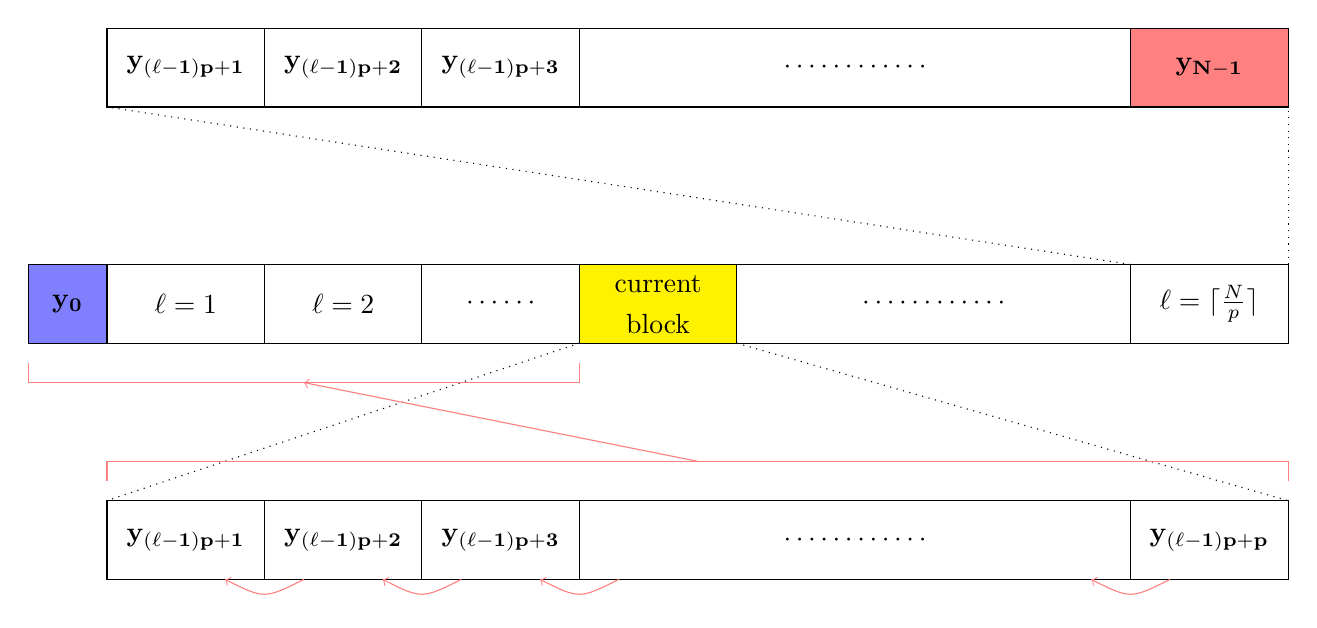
\begin{tikzpicture}
    \filldraw[fill=blue!50] (-1,0) rectangle (0,1);
    \draw (0,0) -- (0,1);
    \draw (-0.5,0.5) node { $ \mathbf{y_0} $ };
    \draw (-1,0) -- (15,0) -- (15, 1) -- (-1, 1) -- cycle;
    \draw (2,0) -- (2,1);
    \draw (4,0) -- (4,1);
    \draw (1,0.5) node { $ \ell = 1 $ };
    \draw (3,0.5) node { $ \ell = 2 $ };
    \draw (5,0.5) node { $ \cdots \cdots $ };
    \draw (6,0) -- (6,1);
    \draw (8,0) -- (8,1);
    \draw (10.5,0.5) node { $ \cdots \cdots \cdots \cdots  $ };
    \draw (13,0) -- (13,1);
    \draw (14,0.5) node { $ \ell = \lceil \frac{N}{p} \rceil $ };
    \filldraw[fill=yellow] (6,0) rectangle (8,1);
    \draw (7,0.75) node { current };
    \draw (7,0.25) node { block };
    \draw [dotted] (6,0) -- (0,-2);
    \draw [dotted] (8,0) -- (15,-2);
    \draw (0,-2) -- (15,-2) -- (15,-3) -- (0,-3) -- cycle;
    \draw (2,-3) -- (2,-2);
    \draw (4,-3) -- (4,-2);
    \draw (6,-3) -- (6,-2);
    \draw (13,-3) -- (13,-2);
    \draw (1,-2.5) node { $ \mathbf{ y_{(\ell - 1) p + 1} } $ };
    \draw (3,-2.5) node { $ \mathbf{ y_{(\ell - 1) p + 2} } $ };
    \draw (5,-2.5) node { $ \mathbf{ y_{(\ell - 1) p + 3} } $ };
    \draw (9.5, -2.5) node { $ \cdots \cdots \cdots \cdots $ };
    \draw (14,-2.5) node { $ \mathbf{ y_{(\ell - 1) p + p} } $ };
    \draw [dotted] (13,1) -- (0,3);
    \draw [dotted] (15,1) -- (15,3);
    \draw (0,3) -- (15,3) -- (15,4) -- (0,4) -- cycle;
    \draw (2,3) -- (2,4);
    \draw (4,3) -- (4,4);
    \draw (6,3) -- (6,4);
    \filldraw[fill=red!50] (13,3) rectangle (15,4);
    \draw (13,3) -- (13,4);
    \draw (1,3.5) node { $ \mathbf{ y_{(\ell-1)p + 1} } $ };
    \draw (3,3.5) node { $ \mathbf{ y_{(\ell-1)p + 2} } $ };
    \draw (5,3.5) node { $ \mathbf{ y_{(\ell-1)p + 3} } $ };
    \draw (9.5,3.5) node { $ \cdots \cdots \cdots \cdots $ };
    \draw (14,3.5) node { $ \mathbf{ y_{N-1} } $ };
    \draw [color=red!50, arrows={->}] (13.5,-3) .. controls (13,-3.25) .. (12.5,-3); 
    \draw [color=red!50, arrows={->}] (6.5,-3) .. controls (6,-3.25) .. (5.5,-3); 
    \draw [color=red!50, arrows={->}] (4.5,-3) .. controls (4,-3.25) .. (3.5,-3);    
    \draw [color=red!50, arrows={->}] (2.5,-3) .. controls (2,-3.25) .. (1.5,-3);
    \draw [color=red!50] (-1,-0.25) -- (-1,-0.5) -- (6,-0.5) -- (6,-0.25);
    \draw [color=red!50] (0,-1.75) -- (0,-1.5) -- (15,-1.5) -- (15,-1.75);
    \draw [color=red!50, arrows={->}] (7.5,-1.5) -- (2.5, -0.5);
\end{tikzpicture}

    \caption{Computation diagram for the values in the vector (array) $ \mathbf{y} $.}
\end{figure} The centre row shows how $ \mathbf{y} $ is broken up into blocks, and the bottom row is a detailed view
of the contents of the \emph{current block} being computed.
The red lines indicate dependency, in that $ \mathbf{y}_{(\ell - 1)p + 1} $ depends on all the $ y_j $ values calculated in the previous blocks. $ \mathbf{y}_{(\ell - 1)p + 2} $ depends on all the $ y_j $ values calculated in previous blocks \emph{and} on $ \mathbf{y}_{(\ell - 1)p + 1 } $. 

The idea is that in each block we can do all of the computations which only depend on previous blocks in parallel and then perform the calculations which are dependent on other values within the same block in sequence. After all the values in a particular block are calculated we move on to the next block and repeat the process.

An exploded view of the last block is also provided to emphasise the fact that this block might not contain $ p $ variables if $ p $ does not divide $ N - 1 $. This fact causes us no bother as it is easy to handle in code.

As in \cite{Diethelm2011} we rewrite the sums \eqref{eq:AMB_Predictor} and $ \eqref{eq:AMB_y} $ as 
\begin{align}
    y_{j+1}^P = I_{j+1} + h^\alpha H_{j,\ell}^P + h^\alpha L_{j,\ell}^P
\end{align}
and
\begin{align}
    y_{j+1} = I_{j+1} + h^{\alpha} H_{j,\ell} + h^\alpha L_{j,\ell}
\end{align}

where 
\begin{align}
    I_{j+1}         & := \sum_{k=0}^{\lceil \alpha \rceil -1} \frac{x_{j+1}^k}{k!} y_0^{(k)} \\
    H^P_{j,\ell}    & := \sum_{k=0}^{(\ell-1)p} b_{j-k} f(x_k, y_k) \\
    L_{j,\ell}^P    & := \sum_{k=(\ell-1)p+1}^{j} b_{j-k} f(x_k,y_k) \\
    H_{j,\ell}      & := c_j f(x_0, y_0) + \sum_{k=1}^{(\ell - 1)p} a_{j-k}f(x_k, y_k) \\
    L_{j,\ell}      & := \sum_{k=(\ell-1)p + 1}^j a{j-k} f(x_k, y_k) + \frac{f(x_{j+1}, y^P_{j+1})}{\Gamma(\alpha + 2.)}
\end{align}
In each block the values of $ H, I $ and $ H^P $ can be calculated in parallel for each $ y_j $ in the block.Then there is a somewhat more complex dependency between these sums. 

To best explain how the processes procedes in each block and what dependencies there are we will consider a specific example where there are two values to be calculated per block (i.e. $ p = 2 $). Consider figure \ref{fig:AMB_Task_Flow}. 

Each box in the figure represents a task. A task can execute when all the tasks with arrows pointing to it have completed. The little red number represents the index of the variable \emph{within} the block which is being calculated. All the task names are reasonablly self explanatory except for perhaps $ S^P $ and $ S $. These take the values calculated in the other sums and add them together to get $ y^P $ and $ y $ respectivly. These are very small tasks which take very little time to execute.

The red arrow illustrate the interdependency of variables within a block. The second variable cannot have the sum $ L^P $ calculate until the first variable is calculated. This means that in effect each of the $ L $ tasks have to execute in series but these sums are relatively small so the time taken is quite short. Each block is then executed in sequence as each block depends on the blocks before it. See Appendix A for a C\# implementation of this. 

\begin{figure}[H]
    %PID Controller Closed Loop Diagram.
\begin{tikzpicture} 
    \draw (10,20) -- (13,20) -- (13, 19) -- (10, 19) -- cycle;
    \draw (11.5,19.5) node { Block Start };
    \draw (11.5, 19) -- (11.5, 18);
    \draw (4.5, 18) -- (19.5, 18);
    \draw [->] (4.5, 18) -- (4.5, 17);
    \draw [->] (7.5, 18) -- (7.5, 17);
    \draw [->] (10.5, 18) -- (10.5, 17);
    \draw [->] (11.5, 18) -- (11.5, 13) -- (10, 13);
    \draw (3.75, 17) -- (5.25, 17) -- (5.25, 15.5) -- (3.75, 15.5) -- cycle;
    \draw (6.75, 17) -- (8.25, 17) -- (8.25, 15.5) -- (6.75, 15.5) -- cycle;
    \draw (9.75, 17) -- (11.25, 17) -- (11.25, 15.5) -- (9.75, 15.5) -- cycle;
    \draw (8.5, 12.25) -- (10, 12.25) -- (10,13.75) -- (8.5, 13.75) -- cycle;
    \draw (7.5, 14.5) -- (10.5, 14.5);
    \draw [->] (4.5, 15.5) -- (4.5, 4.25) -- (8.5, 4.25);
    \draw (7.5, 14.5) -- (7.5, 15.5);
    \draw (10.5, 14.5) -- (10.5, 15.5);
    \draw (7.5, 15.5) -- (7.5, 10);
    \draw [->] (7.5, 10) -- (8.5, 10);
    \draw (8.5, 9.25) -- (8.5, 10.75) -- (10, 10.75) -- (10, 9.25) -- cycle;
    \draw [->] (9.25, 12.25) -- (9.25, 10.75);
    \draw [->] (9.25, 9.25) -- (9.25, 8);
    \draw (8.5, 8) -- (10, 8) -- (10, 6.5) -- (8.5, 6.5) -- cycle ;
    \draw [->] (9.25, 6.5) -- (9.25, 5);
    \draw (8.5, 5) -- (8.5, 3.5) -- (10, 3.5) -- (10, 5) -- cycle;
    \draw [->] (18.5, 18) -- (18.5, 17);
    \draw [->] (15.5, 18) -- (15.5, 17);
    \draw [->] (12.5, 18) -- (12.5, 17);
    \draw (11.75, 17) -- (13.25, 17) -- (13.25, 15.5) -- (11.75, 15.5) -- cycle;
    \draw (14.75, 17) -- (16.25, 17) -- (16.25, 15.5) -- (14.75, 15.5) -- cycle;
    \draw (17.75, 17) -- (19.25, 17) -- (19.25, 15.5) -- (17.75, 15.5) -- cycle;
    \draw [->] (12.5, 15.5) -- (12.5, 4.25) -- (16.5, 4.25);
    \draw [->] (19.5, 18) -- (19.5, 13) -- (18, 13);
    
    
    \draw (15.5, 14.5) -- (18.5, 14.5);
    \draw [->] (12.5, 15.5) -- (12.5, 4.25) -- (16.5, 4.25);
    \draw (15.5, 14.5) -- (15.5, 15.5);
    \draw (18.5, 14.5) -- (18.5, 15.5);
    \draw (15.5, 15.5) -- (15.5, 10);
    \draw [->] (15.5, 10) -- (16.5, 10);
    \draw (16.5, 9.25) -- (16.5, 10.75) -- (18, 10.75) -- (18, 9.25) -- cycle;
    \draw [->] (17.25, 12.25) -- (17.25, 10.75);
    \draw [->] (17.25, 9.25) -- (17.25, 8);
    \draw (16.5, 8) -- (18, 8) -- (18, 6.5) -- (16.5, 6.5) -- cycle ;
    \draw [->] (17.25, 6.5) -- (17.25, 5);
    \draw (16.5, 5) -- (16.5, 3.5) -- (18, 3.5) -- (18, 5) -- cycle;
    \draw (16.5, 12.25) -- (18, 12.25) -- (18,13.75) -- (16.5, 13.75) -- cycle;
    \draw [color=red, arrows={->}] (10, 4.25) -- (12,4.25) -- (12, 13) -- (16.5, 13);
    \draw (4.5, 16.25) node { $ H $ };
    \draw (5, 15.75) node[color=red]  { $ 1 $ };
    
    \draw (7.5, 16.25) node { $ I $ };
    \draw (8, 15.75) node[color=red]  { $ 1 $ };
    
    \draw (10.5, 16.25) node { $ H_p $ };
    \draw (11, 15.75) node[color=red]  { $ 1 $ };
    
    \draw (9.25, 13) node { $ L_p $ };
    \draw (9.75, 12.5) node[color=red] { $ 1 $ };
    
    \draw (9.25, 10) node { $ S_p $ };
    \draw (9.75, 9.5) node[color=red] { $ 1 $ };
    
    \draw (9.25, 7.25) node { $ L $ };
    \draw (9.75, 6.75) node[color=red] { $ 1 $ };
    
    \draw (9.25, 4.25) node { $ L $ };
    \draw (9.75, 3.75) node[color=red] { $ 1 $ };
    
    
    
    \draw (12.5, 16.25) node { $ H $ };
    \draw (13, 15.75) node[color=red]  { $ 2 $ };
    
    \draw (15.5, 16.25) node { $ I $ };
    \draw (16, 15.75) node[color=red]  { $ 2 $ };
    
    \draw (18.5, 16.25) node { $ H_p $ };
    \draw (19, 15.75) node[color=red]  { $ 2 $ };
    
    \draw (17.25, 13) node { $ L_p $ };
    \draw (17.75, 12.5) node[color=red] { $ 2 $ };
    
    \draw (17.25, 10) node { $ S_p $ };
    \draw (17.75, 9.5) node[color=red] { $ 2 $ };
    
    \draw (17.25, 7.25) node { $ L $ };
    \draw (17.75, 6.75) node[color=red] { $ 2 $ };
    
    \draw (17.25, 4.25) node { $ L $ };
    \draw (17.75, 3.75) node[color=red] { $ 2 $ };
    
    \draw [->] (17.25, 3.5) -- (17.25, 2) -- (11.5, 2) -- (11.5, 1);
    
    \draw (10,1) -- (13,1) -- (13, 0) -- (10, 0) -- cycle;
    \draw (11.5,0.5) node { Block End };
\end{tikzpicture}

    \caption{Task flow diagram for each block in the case when $ p = 2 $}
    \label{fig:AMB_Task_Flow}
\end{figure}

\subsubsection{Application of the Scheme to the Relaxation-Oscilation Equation}
Before continuing to analyse the performance of this method or discuss possible improvements we pause for a moment of intelectual indulgence and apply this scheme to the relaxation-oscilation equation.

We define the (Caputo) relaxation-oscilation equation as
\begin{align}
    \label{eq:relax-oscil}
    \capder{0}{\alpha}{x}{y}(x) = -y(x)
\end{align}
for $ 0 < \alpha \leq 2 $.
along with initial conditions 
\begin{align}
    \label{eq:relax-oscil-ic}
    y(0) = 1, y'(0) = 0, y''(0) = 0
\end{align}

In the case where $ \alpha = 1 $ this results in the well known exponential solution and in the case where $ \alpha = 2 $ this results in the well known trigonometric solution.

In figure \ref{fig:Relax_Oscil} we show a plot of all solutions as $ \alpha $ ranges from $ \frac{1}{2} $ to $ 2 $.

\begin{figure}[H]
    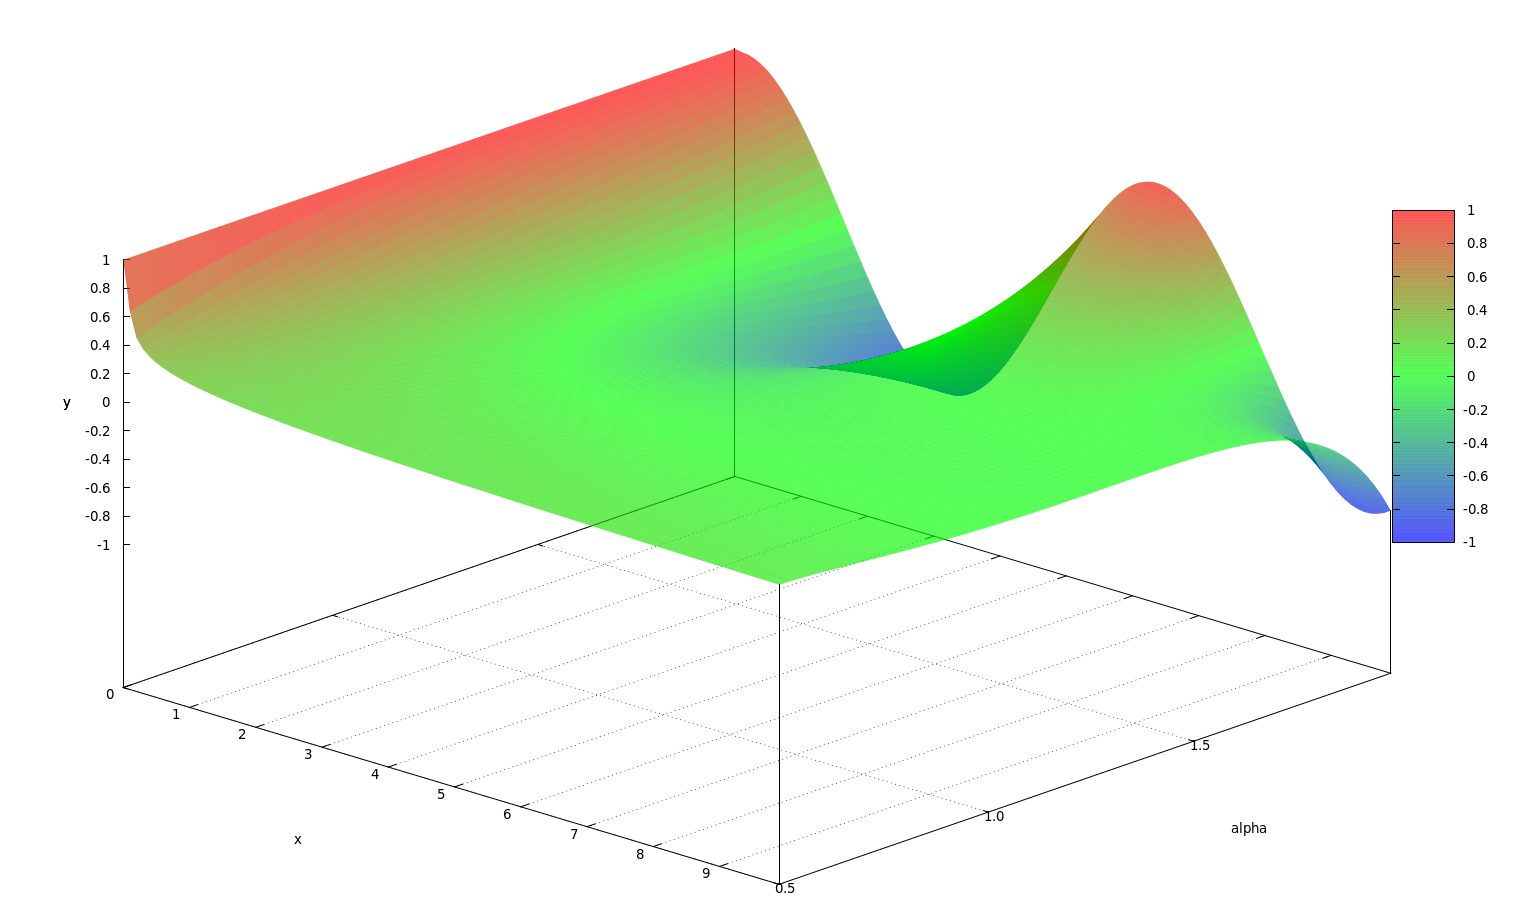
\includegraphics[scale = 0.3]{images/FDE_Solution_Surface_No_Label}
    \caption{Solution surface of the relaxation-oscilation equation defined in \eqref{eq:relax-oscil} and \eqref{eq:relax-oscil-ic}.}
    \label{fig:Relax_Oscil}
\end{figure}


\subsection{Analysis of the Performance of the Scheme in C\# and MONO}

We wish to analyse the performance of this scheme, and specifically its implementation in C\# (MONO). Although this scheme is extremely similar to that outlined in \cite{Diethelm2011} it differs mainly in the fact that this is a task based scheme which does not have an explicit number of threads which are executed. This is because we rely on a task scheduler to do that for us. In this scheme we let $ p $ denote the number of variables per block (and then spawn up to 4 simultaneous tasks per variable) instead of having $ p $ explicit threads for each block. 
As can be seen from the code in Appendix A this results in easy to define dependencies and the bulk of the multithreading logic being done in just 40 lines of code.

A possible drawback of this scheme is that it relies on the a task scheduler which may or may not be optimised for the type of workload being placed on it. We will discuss this issue in more detail later on.

To understand the performance characteristics of this scheme see figure \ref{fig:mono_performance_surface} for a \emph{performance surface} which shows the average runtime of the scheme for different values of $ p $ and $ N $.

\begin{figure}[H]
    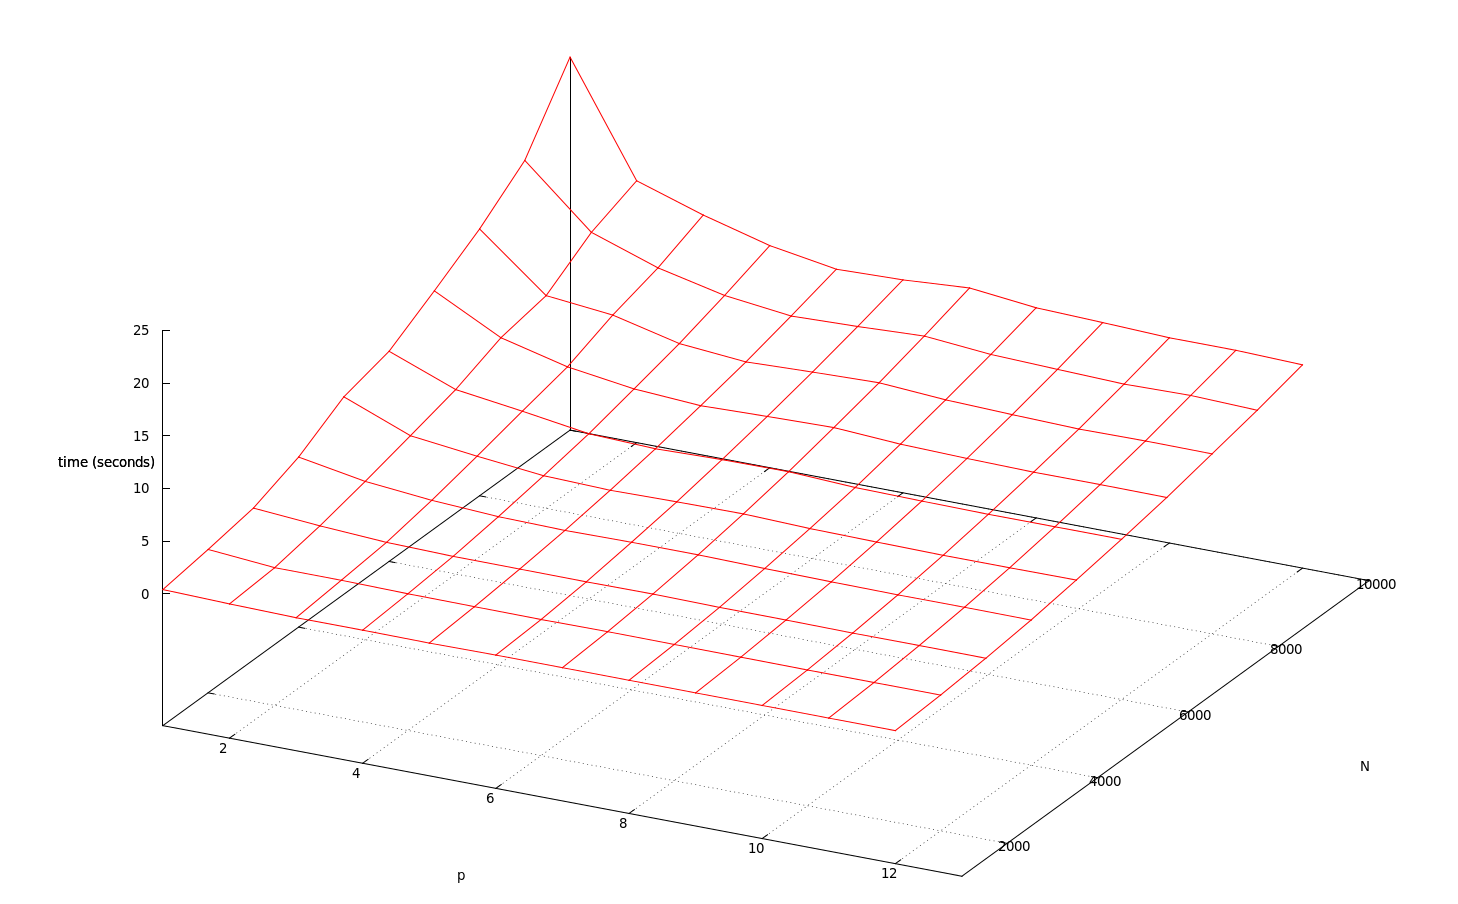
\includegraphics[scale = 0.3]{images/Dot_Net_Performance_No_Label}
    \caption{Average runtime of the scheme for different values of $ p $ and $ N $}
    \label{fig:mono_performance_surface}
\end{figure}

Firstly the $ O(N^2) $ complexity of the algorithm is quite clearly visible, especially in the case where $ p = 1 $. Secondly the law of diminishing returns is also clearly visible in this plot. In the case where $ p = 1 $ it should be noted that there are up to $ 4 $ tasks running just for that one variable ($ I $, $ L^P $, $ H $, $ H^P $). In \cite{Diethelm2011} $ p = 1 $ would refer to only 1 thread running at all times, which is not the case here. This is has its advantages and disadvantages.  Its clearly advantageous because it results in potentially higher concurrency but disadvantageous because it limits out ability to compare this scheme with the one in \cite{Diethelm2011} on a \emph{thread for thread} basis. 

It should also be noted that setting large values for $ p $ (more than the number of cores available) should not be as bad as it would be in the case where we are dealing with raw threads. The task scheduler will decide what the maximum number of concurrent tasks should be an execute the tasks accordingly. In the case of the default scheduler it may still incur a performance hit because the scheduler may / will spend time task switching to ensure 
